\section{Q-values}

\begin{frame} 
\mode<presentation>{
    \begin{center} \huge
        \secname
    \end{center}  
    }
    \begin{center} 
    values of state-action pairs
    \end{center}
\end{frame}

\begin{frame}

Higher resolution value.

\begin{center}
		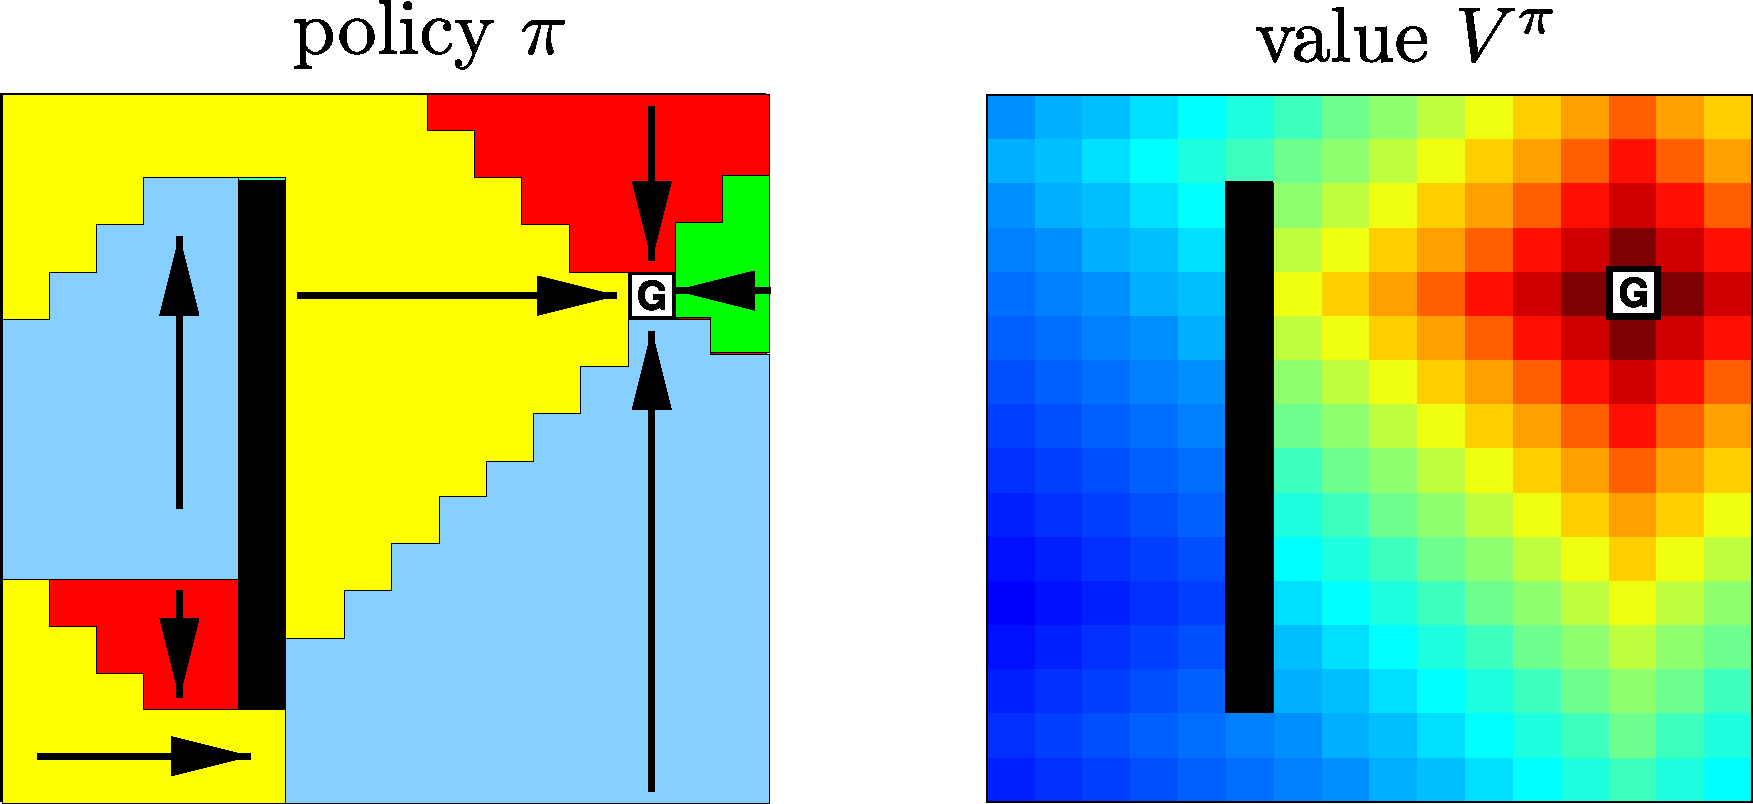
\includegraphics[width=8cm]{img/nav_policy_and_value}
\end{center} 

\begin{center}
		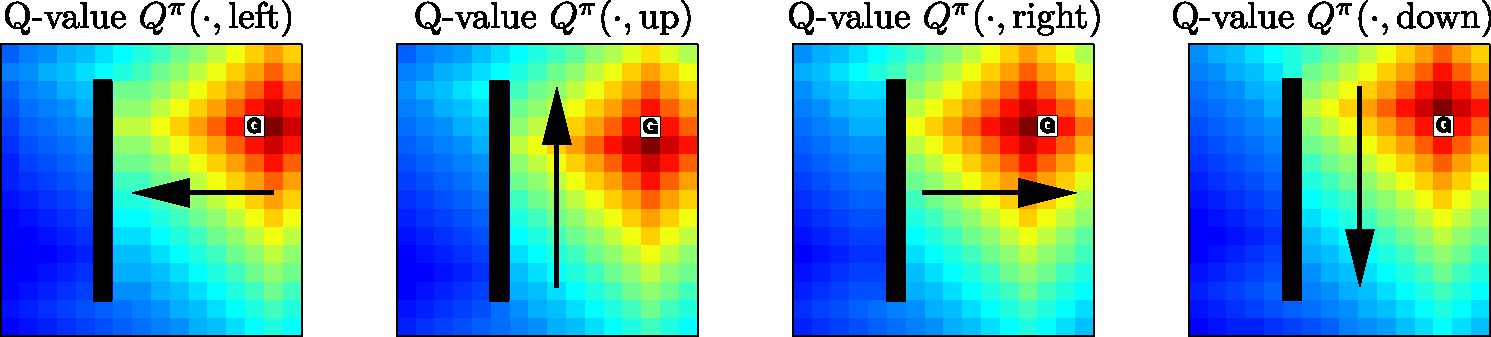
\includegraphics[width=\textwidth]{img/nav_qvalues}
\end{center} 

\end{frame}

\begin{frame}\frametitle{The Q-value function}

\mode<article>{
The Q-values function is defined as:
}
\begin{equation}
		Q^\pi(\vec x_i, \vec a_k) \quad=\quad 
		\E\bigg\lbrack \,
			\smallsum{t=0}\infty \, \gamma^t \,  
				{\color{reward}r(\vec x^{(t)}, \vec a^{(t)})}
			\, \bigg| \begin{array}{l}
				\scriptstyle \vec x^{(0)} =\, \vec x_i \,, \quad 
					\vec a^{(0)} =\, \vec a_k \\[-1mm]
				\scriptstyle {\color{trans} \vec x^{(t+1)} 
					\,\sim\, P(\cdot|\vec x^{(t)}, \vec a^{(t)})}\\[-1mm]
				\scriptstyle {\color{policy} \vec a^{(t+1)} 
				\,\sim\, \pi(\cdot|{\color{trans}\vec x^{(t+1)}})}
			\end{array}	
		\bigg\rbrack
\end{equation}

The state-action value measures the expected return whenever we start at $\vec x_i$ and take action $\vec a_k$ and follow the policy $\pi$ from there.



\end{frame}

\begin{frame}

\mode<presentation>{
\begin{itemize}
\item[] states $\vec x \in \{ \vec x_1, \ldots, \vec x_S\}$, 
actions $\vec a \in \{ \vec a_1, \ldots, \vec a_A\}$,\\
reward function $r(\vec x_i, \vec a_k)$,
\item[]
transition model ${\color{trans} P(\vec x_j | \vec x_i, \vec a_k)}$ and
policy ${\color{policy} \pi(\vec a_k | \vec x_i)}$
\end{itemize}
}

\begin{center}
		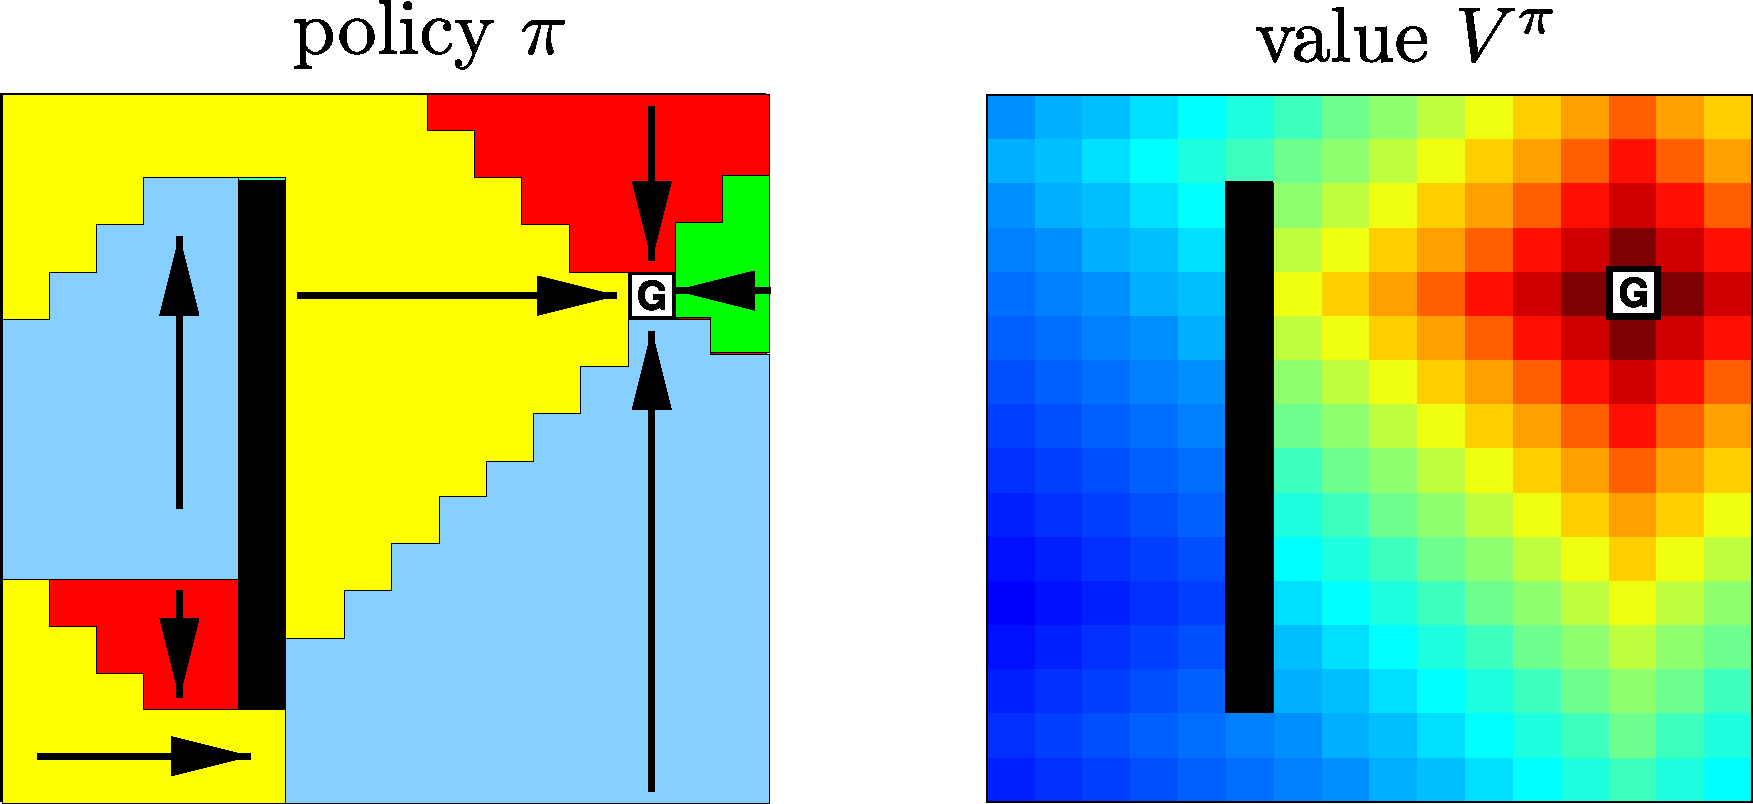
\includegraphics[width=3cm]{img/nav_policy_and_value}
\end{center} 

\begin{center}
		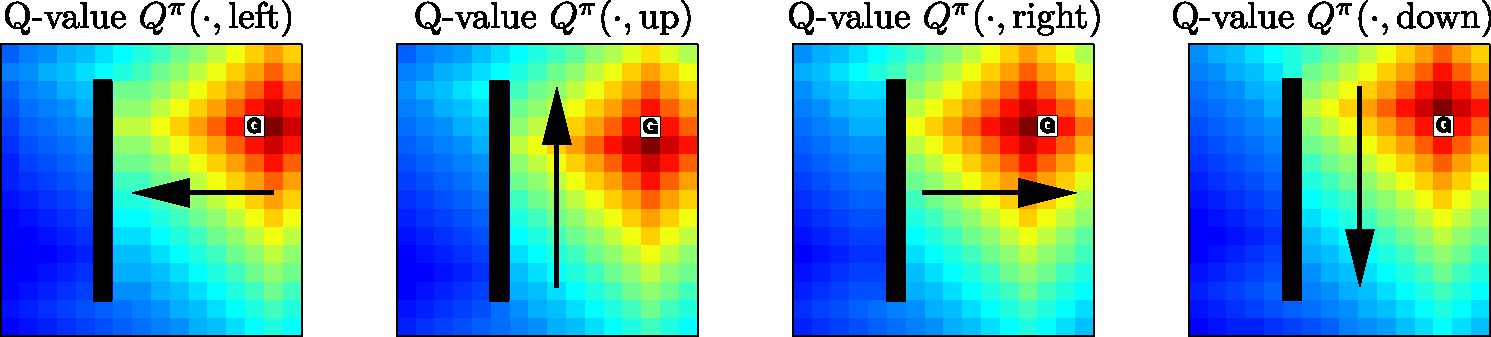
\includegraphics[width=0.7\textwidth]{img/nav_qvalues}
\end{center} 

\question{How does the value function relate to the Q-value function?}

\pause

\slidesonly{\vspace{-7mm}}
\notesonly{- yes, through:}

\begin{equation}
V^\pi(\vec x_i) = \visible<3->{
{\only<4>{\color{policy}}\sum_{k=1}^{A}}
\visible<4>
{\color{policy}
\pi(\vec a_k|\vec x_i)
}
}
\visible<2->{{\color{black}Q^\pi(\vec x, \vec a_k)}}
\end{equation}

\end{frame}

\begin{frame}
	\begin{block}{Reminder: Bellman equation (decomposition) for the value function}
			\begin{equation}
			V^\pi_i
			= {\color{reward}\vec r^\pi_i} 
					+ \gamma {\color{trans}\vec P^\pi_{ij}} \vec v^\pi_{j}
			\end{equation} 
	\end{block}
	
	\begin{block}{Bellman equation (decomposition) for Q-values}
		\vspace{-4mm}	
		\begin{align}
			Q^\pi(\vec x_i, \vec a_k) \;\;&=\;\; 
			{\color{reward} r(\vec x_i, \vec a_k)} \;+\; 
			\gamma {\color{trans} \sum_{j=1}^S 
				P(\vec x_j | \vec x_i, \vec a_k)} \;
				V^\pi({\color{trans}\vec x_j})
			\\
			&=\;\; 
			{\color{reward} r(\vec x_i, \vec a_k)} \;+\; 
			\gamma {\color{trans} \sum_{j=1}^S 
				P(\vec x_j | \vec x_i, \vec a_k)} \;
				{\color{policy} \sum_{l=1}^{A} \, 
					\pi(\vec a_l | {\color{trans}\vec x_j})} \,
					Q^\pi({\color{trans}\vec x_j}, 
						{\color{policy}\vec a_l})
		\end{align}
	\end{block}
\end{frame}
